\chapter{Introduction}

\KOMAoptions{headsepline=true}
\lohead{\leftmark}
\rehead{\rightmark}
\pagenumbering{arabic}
\setcounter{page}{1}


The goal of this PhD project is the development of linear optics measurement methods for
circular accelerators.
The term \emph{optics} is used because the manipulation of a charged particle beam in an accelerator shares
many characteristics with the bending and focusing of light through lenses and other optical
devices and \emph{linear} refers to lattice elements with linear magnetic field.

Linear optics corrections have achieved remarkable performance in the last years %
\cite{Tomas2017, Tomas2012, Persson2017, Aiba2013, Sagan2000, Borer1983, Langner2015},
pushing the precision and accuracy of machine parameters further.
But development of accelerator technology is not resting either and the introduction of
next generation light sources and the design and construction of new colliders and future projects
constantly demand more advanced and precise measurement methods.

Data acquisition and processing, as well as the final analysis and correction procedures, is performed on
electronic devices and computers. Therefore the term \emph{method} used in this work to describe
a measurement or correction procedure, usually encompasses also the implementation of a dedicated computer algorithm.

For the largest machines -- containing thousands of lattice elements -- many classical measurement and
correction methods suffer from long execution times as the computational complexity of the measurement
and correction algorithms grows with the number of parameters, often exponentially. 
Therefore, the speed of the used techniques is also getting more and more crucial for a smooth operation. 
Moreover, often the full potential of the analysis can only be harvested \emph{offline} in the days and
weeks following the actual measurement.

\section{Objectives of this work}

In this work three distinct optics measurement methods are treated. All of these methods take as input the
Fourier analysis of turn-by-turn data of the beam centroid position, picked up at certain measurement
devices called \emph{Beam Position Monitors} (BPMs). In order to get a sufficiently strong signal, the
particle beam is excited. If the excitation method induces a forced oscillation, optics functions are changed
and this effect has to be compensated.
The remainder of this chapter introduces the data acquisition and its surrounding devices, as well as
CERN and its accelerator facilities.

The first method is a more precise and faster 
measurement of the $\beta$~function, an optics parameter that presents a direct observable for the
focusing at any given point in the machine. Constraints on the tolerances of focusing errors are given
for machine performance and protection reasons. An improvement of the classical $\beta$~function measurement
was presented in a previous work. This thesis builds upon this improvement and enhances it in terms of speed
and precision.

The second method is a new local observable for linear lattice imperfections.
In the LHC precise optics correction
methods consider a local region of the accelerator as transfer line. Measured optics functions at the start
of the segment are used as initial condition for a simulation using the best knowledge model of the accelerator.
Then a fitting on the magnetic field strengths is used to match the expected optics to the measured one.
Currently this correction method is used at certain important points in the accelerator where particularly
strict tolerances on errors are given or errors have a high impact on the optics.
Local observables facilitate detecting strong local sources and permit to apply dedicated correction steps.
This work introduces for the first time a local observable for linear lattice errors.

The third topic is the revision and further development of existing methods
to describe the impact of forced particle motion on the measurement of transverse coupling.
Certain lattice elements interlink vertical and horizontal particle motion, an effect called
transverse coupling which has negative impact on the beam stability in the LHC.
The driving device, used to create the signal for turn-by-turn measurements influences
the measurements of certain quantities, including coupling, and this influence has to be compensated.
The current methods neglect a small local effect of this, which became apparent recently.
A new description of the modeling of the driven motion is presented in a previous work and this
thesis applies this description to the measurement of transverse coupling, showing the local
effect for the first time in theoretical considerations.



% --------------------------------------------------------------------------------------------------
% CERN and LHC
% --------------------------------------------------------------------------------------------------
\section{The Large Hadron Collider}

The present work has been carried out mainly at
the \emph{European Organization for Nuclear Research} (CERN)\index{CERN} during commissionning and
machine development studies of
the \emph{Large Hadron Collider} (LHC).
Therefore, this introduction would not be complete without a brief presentation of the used facilities.

The LHC
 is the world's largest particle accelerator with a circumference
of $\SI{27}{\kilo\meter}$. It is situated at the french-swiss border near Geneva as part of
CERN.
The initial purpose of the LHC was to discover the Higgs Boson and to study rare high energy events 
with a centre of mass energy up to $\SI{14}{GeV}$.

The number of collision events is proportional to the \emph{luminosity}\index{luminosity}
%
\begin{equation}
    \mathscr{L} = \frac{N^2 n_b f}{4\pi\sigma_x\sigma_y}
    \label{eq_lumi}
\end{equation}
%
where $N$ is the number of particles per bunch, $n_b$ the number of bunches, $f$ is
the revolution frequency and $\sigma_z$ is the beam size in direction $z$.

\equationref{eq_lumi} assumes that the bunches collide head-on and no deteriorating effects are present. A more realistic form of the luminosity is~\cite{Herr2003}
%
\begin{equation}
    \mathscr{L} = \frac{N^2 n_b f}{4\pi\sigma_x\sigma_y} F
\end{equation}
%
where $F$ is a reduction factor, depending on the exact conditions of the beam and the interaction region such as crossing angle, offset of the beams w.r.t. each other or the optical axis, hourglass effect, non-Gaussian beam profiles etc. In the LHC, $F$ is expected to be around $0.8$. 

The discovery of the Higgs Boson was officially confirmed in 2012~\cite{higgs_1, higgs_2} and since then the
purpose of the LHC lies in providing luminosity for more precise measurements of Higgs channels and
other high energy particle events. 

Particles that enter the LHC are accelerated in several pre-accelerators, forming the so called
\emph{injector chain}\cite{Schindl1999} which is illustrated in \figref{fig_cern_acc_cmplx}.
Protons start their journey as $H^-$ ions in LINAC2 (LINAC4 in the future) where
they are accelerated to $\SI{50}{MeV}$. They are further accelerated in the PS Booster to $\SI{1.4}{GeV}$,
in the Proton Synchroton (PS) to $\SI{25}{GeV}$ and finally to $\SI{450}{GeV}$ in the Super Proton Synchrotron
before they are injected into the LHC.
%
\begin{figure}[ht]
    \centering
    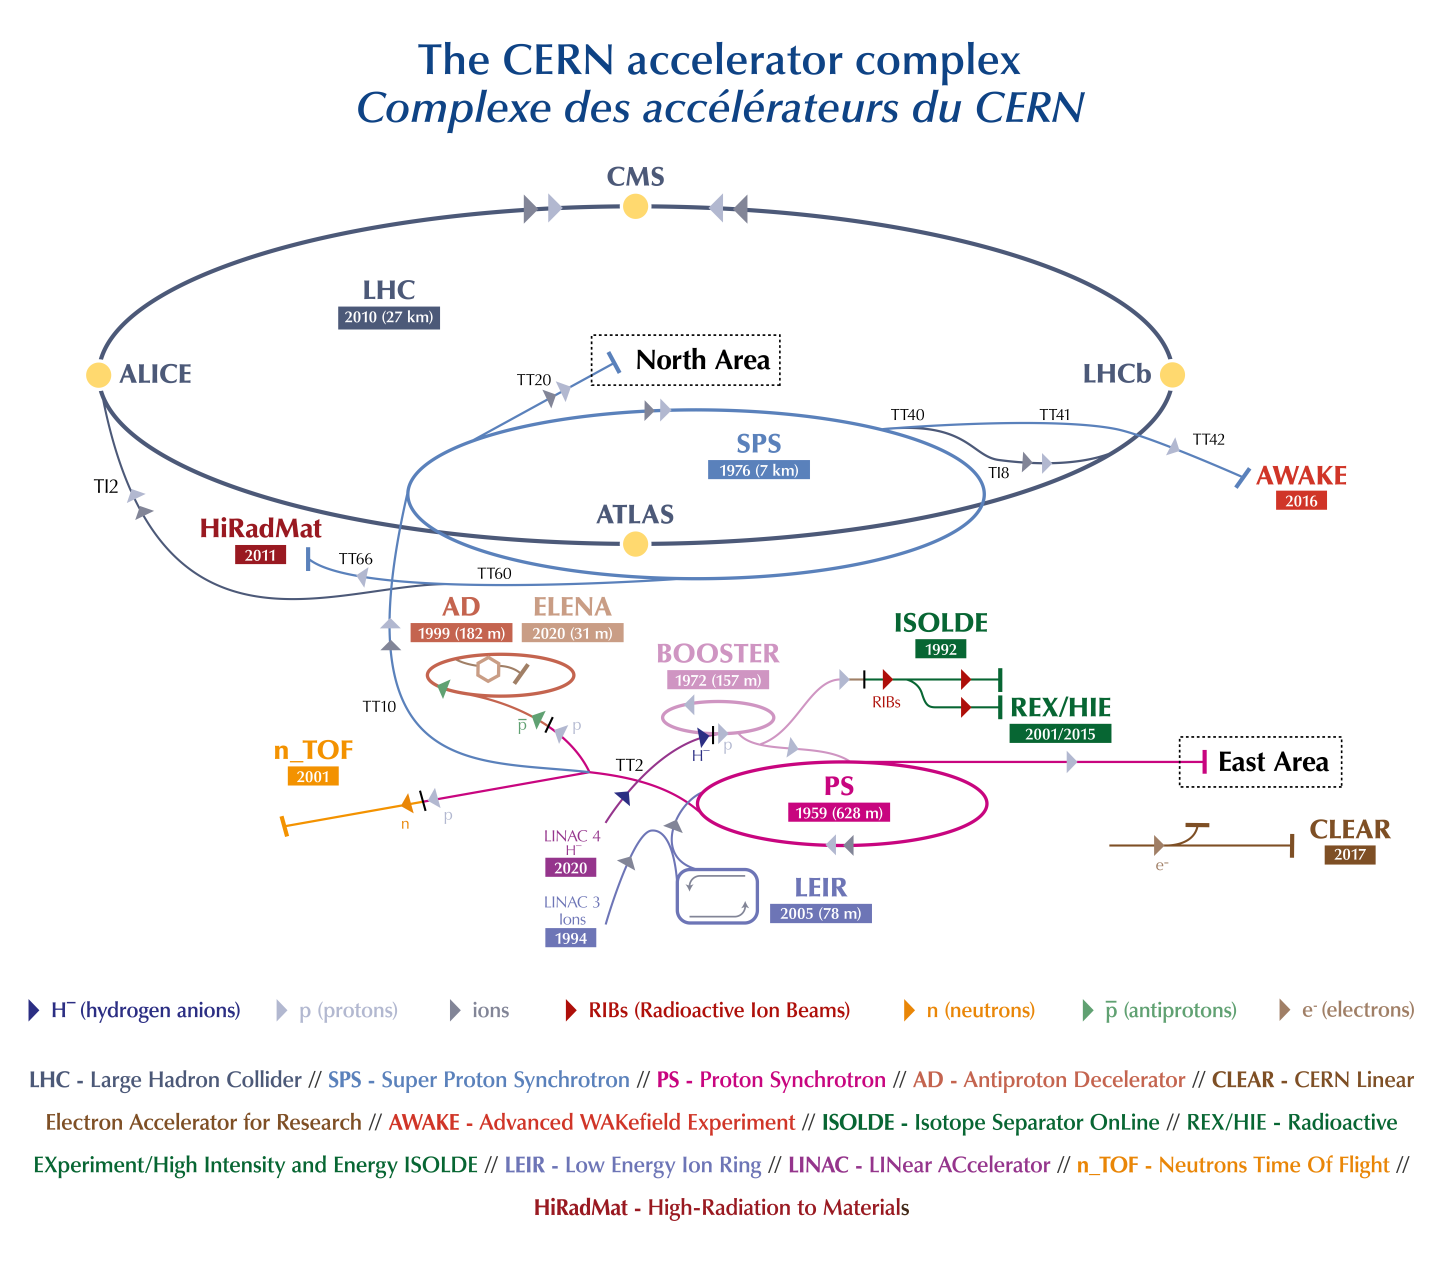
\includegraphics[width=\textwidth]{CCC-v2019-final-white_small}
    \caption{CERN has various accelerators and decelerators. H$^-$ ions are pre-accelerated
    in LINAC2 (LINAC4 in the future) and passed to PSBooster, PS, SPS and finally injected into
    the LHC. Image credit: \cite{CERN_AccCmplx}}
    \label{fig_cern_acc_cmplx}
\end{figure}
%
Heavy ions start in the LINAC3 and are then accelerated in the Low Energy Ion Ring (LEIR) before they are injected into
the PS from where they continue as described for protons.

The LHC consists of eight identical arcs for bending of the beams and eight straight sections between the
arcs which contain the experiments, injection and extraction region and accelerating structures.

An arc consists of 23 so called \emph{FODO}~cells containing two bending sections interleaved with
a focusing and a defocusing quadrupole\footnote{
    The acronym FBDB for focusing-bending-defocusing-bending would be more precise but this work will follow
    the common denomination.
}.
To correct for magnet imperfections, corrector magnets are also installed in the cell.
\figureref{fig_fodo} shows a schematic of an LHC FODO cell.
%
\begin{figure}[ht]
    \centering
    \includestandalone[width=\linewidth]{fodo} 
    \caption{
        Schematic of an LHC FODO cell. Two bending sections, consisting of 3 bending dipoles each
        are interleaved by one focusing and one defocusing quadrupole, respectively.
    }
    \label{fig_fodo}
\end{figure}
%
During long shutdown 2, from 2019 until 2021, the CERN accelerator complex undergoes an extensive upgrade process 
preparing it already partly for the high luminosity upgrade of LHC.
In addition, the injector chain is upgraded in a separate project called \emph{LHC Injector Upgrade} (LIU) \cite{Hanke2017,Bartosik2017}.

% --------------------------------------------------------------------------------------------------
% Intro to OMC
% --------------------------------------------------------------------------------------------------
\section{Optics measurements and corrections}

There are two areas for which the continued measurement and correction of optics parameters is of
importance. The first is machine protection. If the nominal LHC beam hits the wall of the beam pipe
it can deal severe damage to the elements ranging from heating up superconducting elements and
inducing a magnet quench to physically destroying machine parts by melting (or even evaporating) the
material.

The second area for which  optics control is highly important is the machine performance.
The delivered luminosity can be reduced by optics errors.
The two main LHC experiments, ATLAS and CMS demand a luminosity imbalance below $\SI{5}{\percent}$.
To achieve this an optics correction up to the percent level is needed.
High quality optics also improve operational efficiency.

% --------------------------------------------------------------------------------------------------
% Measurement tools and techniques
% --------------------------------------------------------------------------------------------------
\subsection{Measurement tools and techniques}

The most important technique for beam based optics measurements that is applied in the LHC is the excitation
of the particle beam.
If the bunch is excited it performs a betatron oscillation about the closed orbit with a measurable amplitude.
The position of the beam is recorded at certain positions in the accelerator at each revolution. The
obtained turn-by-turn data is then analysed as described later.

To obtain said excitation there are two methods that will be introduced in this section: a free kick
which provokes a free oscillation of the bunch and an AC-dipole which drives a forced oscillation of
the beam. 

% --------------------------------------------------------------------------------------------------
\subsubsection{Free Kick}

If the beam experiences a kick it will perform a damped free oscillation.
The particle's position at the same location turn after turn is illustrated in \figref{fig_kick_plot}.
Light particles like electrons
suffer from a strong damping because of their high synchroton radiation but heavier particles like the
protons accelerated in the LHC are damped much slower.
Nevertheless the oscillation amplitude decreases fast and not many turns are available for high
precision measurements of the turn-by-turn signal. In order to still have as much signal as possible
the kick strength has to be as high as feasible without kicking the beam strongly enough to damage elements or even kick it out of the accelerator.

Furthermore the excitation by a single kick carries the risk of filamenting the
phase space and blowing up the beam emittance.
%
\begin{figure}[ht]
    \centering
    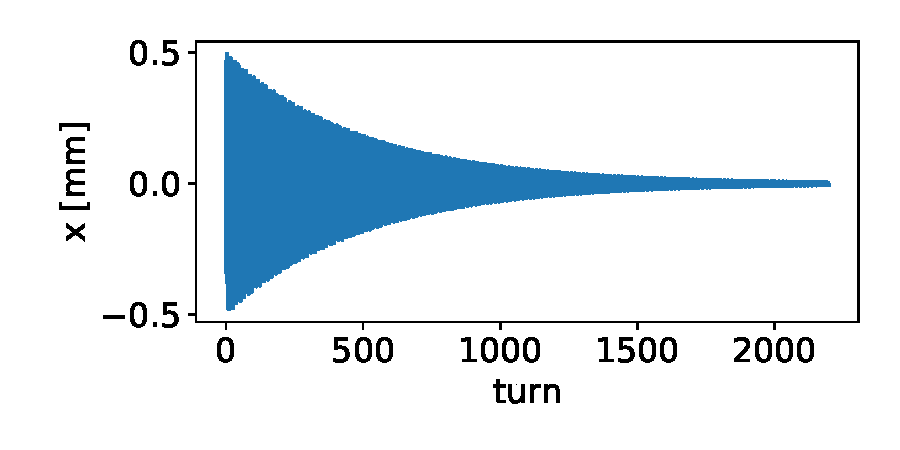
\includegraphics[width=.8\linewidth]{kick_plot.pdf}  
    \caption{The particle's turn-by-turn position for an excitation by a single kick.}
    \label{fig_kick_plot}
\end{figure}
%
\subsubsection{AC-dipole}

The other method to excite the beam that is used in LHC is a dipole connected to an alternating current
power amplifier.
This creates a driven oscillation of the beam \cite{Peggs1998} which can be measured in BPMs \cite{Miyamoto2008, Miyamoto2010}.
The excitation amplitude is slowly ramped up for 2000 turns in order to stay in an
adiabatic regime \cite{Tomas2005ac} held constant for 6600 turns and then again adiabatically ramped down.
The particle's turn-by-turn position is illustrated in \figref{fig_ac_plot}.

The adiabatic ramp up and down prevent a blow up of the beam emittance and since the oscillation amplitude
can be held constant, a smaller maximum amplitude is needed. 
%
\begin{figure}[ht]
    \centering
     \begin{tikzpicture}
    \node (b1) {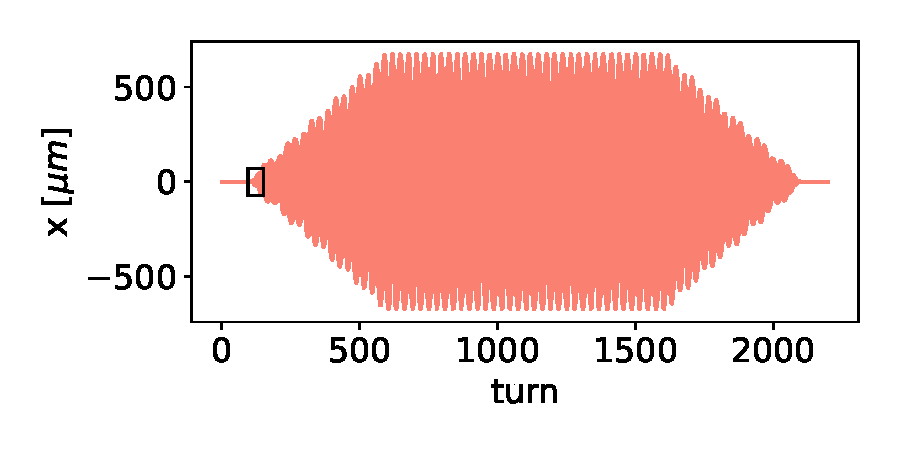
\includegraphics[width=.8\linewidth]{./ac_plot}};
    \node at ($(b1) + (3.2,2.2)$) {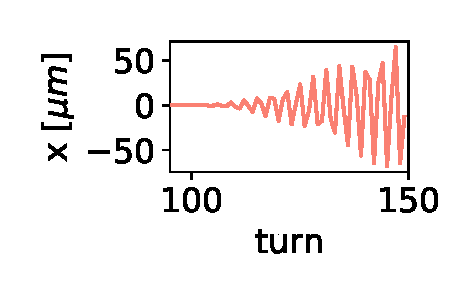
\includegraphics[width=.4\linewidth]{./ac_plot_zoom}};
    \end{tikzpicture}   
    \caption{
        The turn-by-turn position of an AC-dipole excitation. The driving force is ramped up,
        held at flat-top and ramped down again.
        The small plot shows a magnified view of the start of the ramp up.
    }
    \label{fig_ac_plot}
\end{figure}
%
Since the driven excitation creates a forced oscillation as opposed to a free one as in the case of
a single kick, the turn-by-turn motion of the particle does not reflect the pure betatron oscillation
and this effect has to be compensated. For this compensation a good theoretical knowledge of the driven
motion is needed.

%Another disadvantage of the AC-dipole in its current form in the LHC is a cooldown time of about
%one minute that can slow down the measurement process.

% --------------------------------------------------------------------------------------------------
\subsubsection{Beam Position Monitors}

To record the turn-by-turn position of the beam, the LHC possesses more than 500 dual-plane
Beam Position Monitors (BPMs) \cite{koutchouk} which are installed approximately regularly around the ring. 

As the beam passes through the monitor, it induces an electric signal which is then processed
to calculate the beam position.

The BPM resolution in the LHC is approximately $\SI{0.1}{\milli\metre}$ \cite{fcc-bpm,wp2-bpm} with a pilot bunch of
$10^{10}$ protons, that we use to measure the optics.

%The particle's transverse position in Complex Courant-Snyder coordinates at a location $s$ and turn
%$N$ can be optained by applying repeatedly the one turn map:
%%
%\begin{equation}
%    \hat{h}_z^\pm(s + NC) = \sqrt{2J_z} \e{i \left( \varphi_z(s) + 2\pi N Q_z\right)} 
%    \fstop
%\end{equation}
%%
%The real position and momentum of the particle can then be calculated by reversing the steps outlined
%in the first section of this chapter.
%%
%\begin{equation}
%    z(s + NC) = \sqrt{2J_z\beta_z(s)}\cos \left( \varphi_z(s) + 2\pi N Q_z\right)
%\end{equation}
%%
%The phase $\varphi_z(s)$ and amplitude $\sqrt{2J_z\beta_z(s)}$ can be obtained by a Fourier transformation of
%the particle positions.

% --------------------------------------------------------------------------------------------------
% --- Outline
\section{Outline of the thesis}

Chapter~\ref{ch_introduction} gives an introduction of the necessary theory. Starting with linear beam 
dynamics it introduces the most important terminology before passing to the more mathematically involved
regime of normalised coordinates, adding up to the introduction of resonance driving terms which are used
to study beam optics throughout this work.
This formalism is then used to express the quantities needed in later chapters in a useful form. 
Finally, the actual methods used to measure some machine parameters are described in detail giving the
reader an insight into where the newly developed methods will act.
No new discovery is presented in this chapter and it is a mere summary of the theoretical foundations.
Only subsection~\ref{sec_driven_coords} bears a minor amount of original work re-deriving the final form
of the forced coordinates in the used formalism, generalising it to an arbitrary position in the ring.

Chapter~\ref{ch_anbpm} presents the improved $\beta$~function measurement. Previous methods are presented
as well as theoretical foundations of generalised least squares minimisation.
Original studies are presented in the form of a derivation of the analytical error propagation as well as 
simulation studies to assess the speed, accuracy and precision of the new method and experimental
measurements carried out at the LHC.

In chapter~\ref{ch_localobs} a new local observable is derived, use cases and limitations are worked out and
simulations as well as experimental verification are presented. This chapter consists in its entirety of 
original work.

The final topic is presented in chapter~\ref{ch_forced_coupling}. The original work consists of the
derivation of forced coupling resonance driving terms and the comparing studies. For completeness,
methods currently used to model the effect of driven oscillation on the coupling terms are reviewed.
This revision does not represent original work.

Since this thesis treats very distinct topics, each chapter begins with a brief descriptive block to guide
the reader into the respective topic. A brief summary of the chapter's structure is given as well as
an outline of the original work presented in the chapter. 

Finally, chapter~\ref{ch_conclusion} represents a conclusion of the thesis,
summarising the treated topics and highlighting their merit as well as an outlook of further development possibilities.